\documentclass[aspectratio=169,10pt]{beamer}

\usepackage{amsmath,amssymb,amsfonts}
\usepackage{graphicx}
\usepackage{booktabs}
\usepackage{xcolor}
\usepackage{tikz}

% Color Palette: Deep Navy, Teal, Slate
\definecolor{navybg}{HTML}{0A192F}
\definecolor{headernavy}{HTML}{1E3A8A}
\definecolor{accentteal}{HTML}{0D9488}
\definecolor{accentcyan}{HTML}{06B6D4}
\definecolor{accentorange}{HTML}{EA580C}
\definecolor{cardbg}{HTML}{F8FAFC}
\definecolor{cardborder}{HTML}{CBD5E1}
\definecolor{subgray}{HTML}{64748B}

\setbeamercolor{background canvas}{bg=white}
\setbeamercolor{normal text}{fg=black}
\setbeamertemplate{navigation symbols}{}

\title{\textbf{Bayesian Modelling of Wildlife Occurrence Using Camera-Trap Data}}
\subtitle{Estimating Latent Presence, Imperfect Detection, and Community Shrinkage}
\author{\textbf{Aklanta Borah \qquad Amartya Amritanshu \qquad Rajveer Vora}}
\institute{Indian Statistical Institute, Kolkata}
\date{November 2026}

\begin{document}

% ---------------------------------------------------------
% Slide 1: Title Slide (Deep Navy)
% ---------------------------------------------------------
{
\setbeamercolor{background canvas}{bg=navybg}
\begin{frame}[c,plain]
  \centering
  {\scriptsize \textbf{\color{accentcyan} INDIAN STATISTICAL INSTITUTE, KOLKATA}}\\[0.25cm]
  {\Large \textbf{\color{white} Bayesian Modelling of Wildlife Occurrence}}\\[0.15cm]
  {\large \textbf{\color{white} Using Camera-Trap Data}}\\[0.25cm]
  {\small \color{white!80} Latent Presence, Imperfect Detection, and Hierarchical Community Shrinkage}\\[0.60cm]
  {\scriptsize \color{white!60} Aklanta Borah \qquad Amartya Amritanshu \qquad Rajveer Vora}\\[0.10cm]
  {\scriptsize \color{white!40} November 2026}
\end{frame}
}

% ---------------------------------------------------------
% Slide 2: The Core Problem: Non-Detection != Absence
% ---------------------------------------------------------
\begin{frame}[c]
  \begin{center}
    {\large \textbf{\color{headernavy} The Ecological Challenge: Imperfect Detection}}\\[0.08cm]
    {\scriptsize \color{subgray} Why raw camera-trap photographs cannot be treated as census presence records.}
  \end{center}
  \vspace{0.25cm}
  
  \begin{columns}[t,onlytextwidth]
    \begin{column}{0.48\textwidth}
      \setlength{\fboxrule}{1pt}
      \fcolorbox{headernavy!40}{cardbg}{
        \begin{minipage}{\dimexpr\linewidth-2\fboxsep-2\fboxrule\relax}
          \vspace{0.08cm}
          {\small \textbf{\color{headernavy} What We Observe: Photographs}}\\[0.08cm]
          {\scriptsize
          \begin{itemize}
            \setlength{\itemsep}{0.08cm}
            \item Camera traps take photos when motion/heat sensors trigger.
            \item Binary detection $Y_j = 1$ if species is photographed at station $j$.
            \item If no photos occur, $Y_j = 0$.
            \item \textbf{Naive Assumption:} $Y_j = 0 \implies \text{Species is Absent}$.
          \end{itemize}}
          \vspace{0.08cm}
        \end{minipage}
      }
    \end{column}
    
    \begin{column}{0.48\textwidth}
      \setlength{\fboxrule}{1pt}
      \fcolorbox{accentorange!40}{cardbg}{
        \begin{minipage}{\dimexpr\linewidth-2\fboxsep-2\fboxrule\relax}
          \vspace{0.08cm}
          {\small \textbf{\color{accentorange} Physical Reality: Latent State}}\\[0.08cm]
          {\scriptsize
          When $Y_j = 0$, two distinct states are possible:
          \begin{enumerate}
            \setlength{\itemsep}{0.06cm}
            \item \textbf{True Absence ($Z_j = 0$):} Species does not live there.
            \item \textbf{False Absence ($Z_j = 1, Y_j = 0$):} Animal lives there, but walked behind the lens or missed sensor.
          \end{enumerate}
          \textbf{The Consequence:}\\
          Naive detection frequency strictly underestimates true occurrence!}
          \vspace{0.08cm}
        \end{minipage}
      }
    \end{column}
  \end{columns}
  
  \vspace{0.25cm}
  \begin{center}
    \setlength{\fboxrule}{1pt}
    \fcolorbox{cardborder}{cardbg}{
      \parbox{0.94\textwidth}{\centering
        \scriptsize \textbf{\color{headernavy} The Core Question: }
        \textit{How can we mathematically separate true latent presence ($Z$) from conditional detection efficiency ($p$) using repeated sampling occasions?}
      }
    }
  \end{center}
\end{frame}

% ---------------------------------------------------------
% Slide 3: Methodological Bridge: Tanks to Camera Traps
% ---------------------------------------------------------
\begin{frame}[c]
  \begin{center}
    {\large \textbf{\color{headernavy} Methodological Bridge: From German Tanks to Wildlife}}\\[0.08cm]
    {\scriptsize \color{subgray} How discrete latent parameter inference connects wartime intelligence to modern ecology.}
  \end{center}
  \vspace{0.25cm}
  
  \begin{center}
    \resizebox{0.95\linewidth}{!}{
    \begin{tabular}{lll}
      \toprule
      \textbf{Component} & \textbf{The German Tank Problem} & \textbf{Camera-Trap Occupancy Modeling} \\
      \midrule
      \textbf{Unknown Target}     & Discrete population ceiling $N \in \mathbb{N}$ & Latent binary occupancy $Z_j \in \{0, 1\}$ \\
      \textbf{Observed Data}       & Sample serial numbers $\{s_1, \dots, s_k\}$    & Detection history matrix $Y_{jk} \in \{0, 1\}$ \\
      \textbf{Observation Filter}  & Incomplete sample ($m < N$)                   & Imperfect detection trial ($P(Y=1 \mid Z=1) = p < 1$) \\
      \textbf{Naive Pitfall}       & Sample maximum $m$ (downward bias)            & Naive detection rate $s/n$ (underestimates range) \\
      \textbf{Bayesian Solution}   & Marginalize over discrete parameter space     & Marginalize latent mixture: $\psi(1-p)^K + (1-\psi)$ \\
      \bottomrule
    \end{tabular}}
  \end{center}
  
  \vspace{0.25cm}
  \begin{center}
    \setlength{\fboxrule}{1pt}
    \fcolorbox{cardborder}{cardbg}{
      \parbox{0.94\textwidth}{\centering
        \scriptsize \textbf{\color{headernavy} Conceptual Unification: }
        In both problems, classical plug-in estimators fail because the observation process is censored. Bayesian methods solve both by placing probabilistic priors on the latent truth and updating via conditional likelihoods.
      }
    }
  \end{center}
\end{frame}

% ---------------------------------------------------------
% Slide 4: Empirical Dataset: Wildlife Insights
% ---------------------------------------------------------
\begin{frame}[c]
  \begin{center}
    {\large \textbf{\color{headernavy} Empirical Dataset: Wildlife Insights (Cafe Fauna, Peru)}}\\[0.08cm]
    {\scriptsize \color{subgray} Public standardized camera-trap survey from the Alto Mayo protected landscape.}
  \end{center}
  \vspace{0.15cm}
  
  \begin{columns}[c,onlytextwidth]
    \begin{column}{0.48\textwidth}
      {\small \textbf{\color{headernavy} Survey Structure \& Effort}}\\[0.06cm]
      {\scriptsize
      \begin{itemize}
        \setlength{\itemsep}{0.06cm}
        \item \textbf{118 Camera Stations} in coffee agroforestry and montane forest reserves.
        \item \textbf{4,601 Trap-Nights} (median 39.0 days/station; range 8--62 days).
        \item \textbf{109,809 Verified Photographs} (64.9\% blanks; remaining 38.5k verified).
      \end{itemize}}
      \vspace{0.08cm}
      {\small \textbf{\color{accentteal} Five Focal Mammalian Taxa}}\\[0.06cm]
      {\scriptsize
      \begin{itemize}
        \setlength{\itemsep}{0.04cm}
        \item \textbf{Common Opossum}: 74 sites ($62.7\%$), 2,334 imgs.
        \item \textbf{Tapeti}: 31 sites ($26.3\%$), 3,388 imgs.
        \item \textbf{Black Agouti}: 16 sites ($13.6\%$), 402 imgs.
        \item \textbf{Spotted Paca}: 13 sites ($11.0\%$), 435 imgs.
        \item \textbf{Nine-banded Armadillo}: 13 sites ($11.0\%$), 269 imgs.
      \end{itemize}}
    \end{column}
    
    \begin{column}{0.50\textwidth}
      \centering
      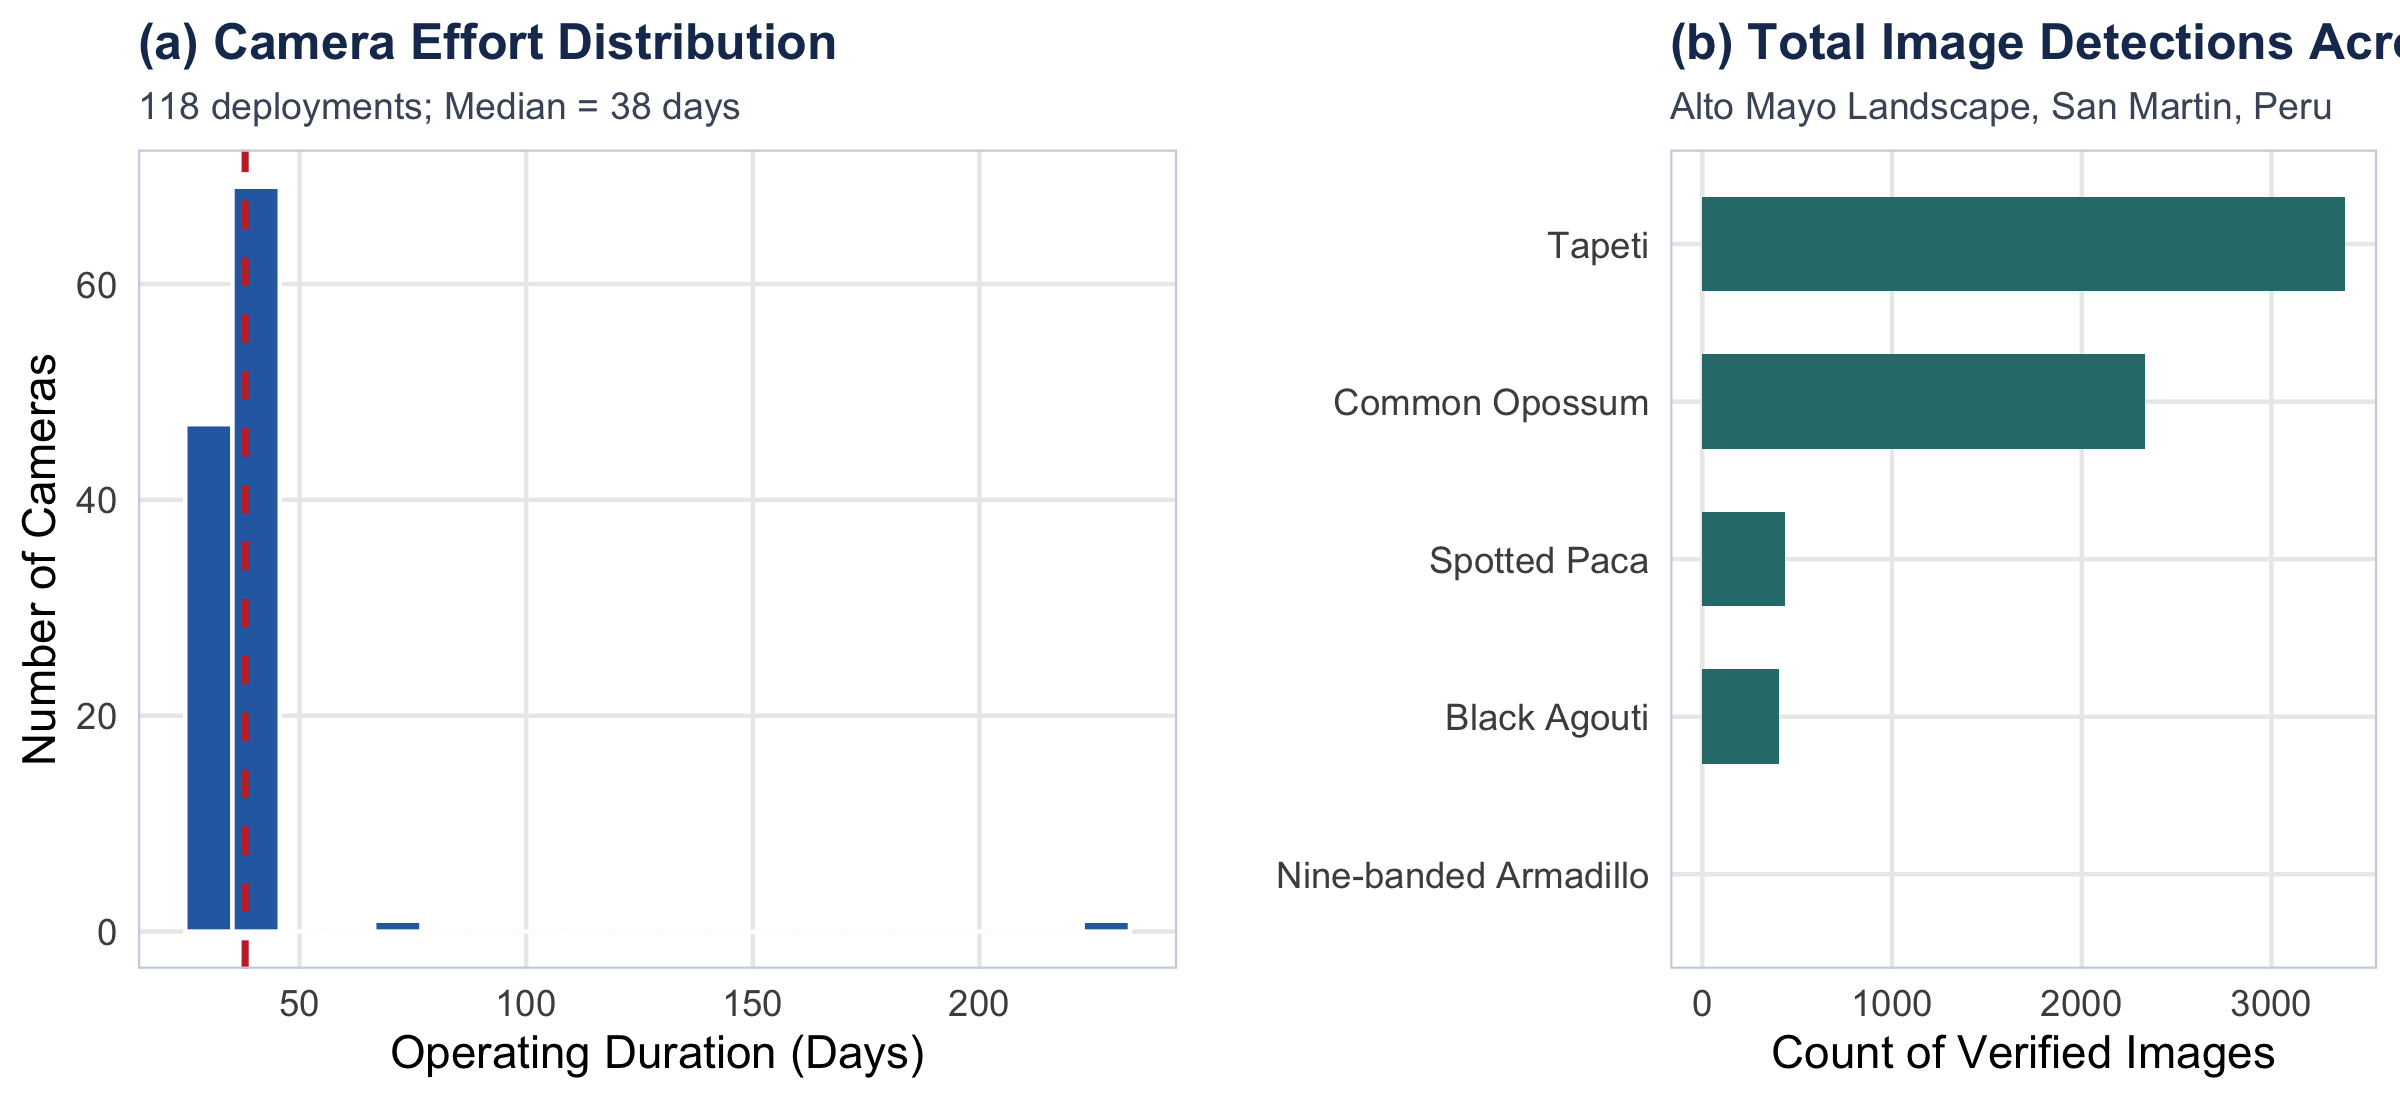
\includegraphics[width=\linewidth]{figures/fig1_eda_species_effort.png}
    \end{column}
  \end{columns}
\end{frame}

% ---------------------------------------------------------
% Slide 5: Section 01 Divider
% ---------------------------------------------------------
{
\setbeamercolor{background canvas}{bg=navybg}
\begin{frame}[c,plain]
  \centering
  {\scriptsize \textbf{\color{accentcyan} SECTION 01}}\\[0.25cm]
  {\LARGE \textbf{\color{white} Conjugate Bayesian Foundations}}\\[0.35cm]
  {\small \color{white!80} Beta--Bernoulli Occurrence, Poisson--Gamma Event Rates, and Prior Sensitivity}
\end{frame}
}

% ---------------------------------------------------------
% Slide 6: Beta-Bernoulli Conjugate Occurrence Model
% ---------------------------------------------------------
\begin{frame}[c]
  \begin{center}
    {\large \textbf{\color{headernavy} Beta--Bernoulli Occurrence \& Prior Sensitivity}}\\[0.08cm]
    {\scriptsize \color{subgray} Exact posterior updating for naive occurrence probability across 118 camera stations.}
  \end{center}
  \vspace{0.15cm}
  
  \begin{columns}[c,onlytextwidth]
    \begin{column}{0.45\textwidth}
      {\small \textbf{\color{headernavy} Analytical Formulation}}\\[0.06cm]
      {\scriptsize
      \begin{itemize}
        \setlength{\itemsep}{0.06cm}
        \item Likelihood: $Y_j \sim \text{Bernoulli}(p)$, $s = \sum Y_j$.
        \item Prior: $p \sim \text{Beta}(\alpha, \beta)$.
        \item Posterior: $p \mid Y \sim \text{Beta}(\alpha + s, \beta + n - s)$.
      \end{itemize}
      \vspace{0.06cm}
      \textbf{Priors Tested:}
      \begin{itemize}
        \setlength{\itemsep}{0.04cm}
        \item \textbf{Flat:} $\text{Beta}(1, 1)$ (Uniform reference)
        \item \textbf{Jeffreys:} $\text{Beta}(0.5, 0.5)$ (Fisher invariant)
        \item \textbf{Conservative:} $\text{Beta}(2, 10)$ (Skeptical of rarity)
      \end{itemize}
      \textbf{Takeaway:} Common taxa ($s=74$) are likelihood-dominated; rare taxa ($s=13$) exhibit mild shrinkage.}
    \end{column}
    
    \begin{column}{0.54\textwidth}
      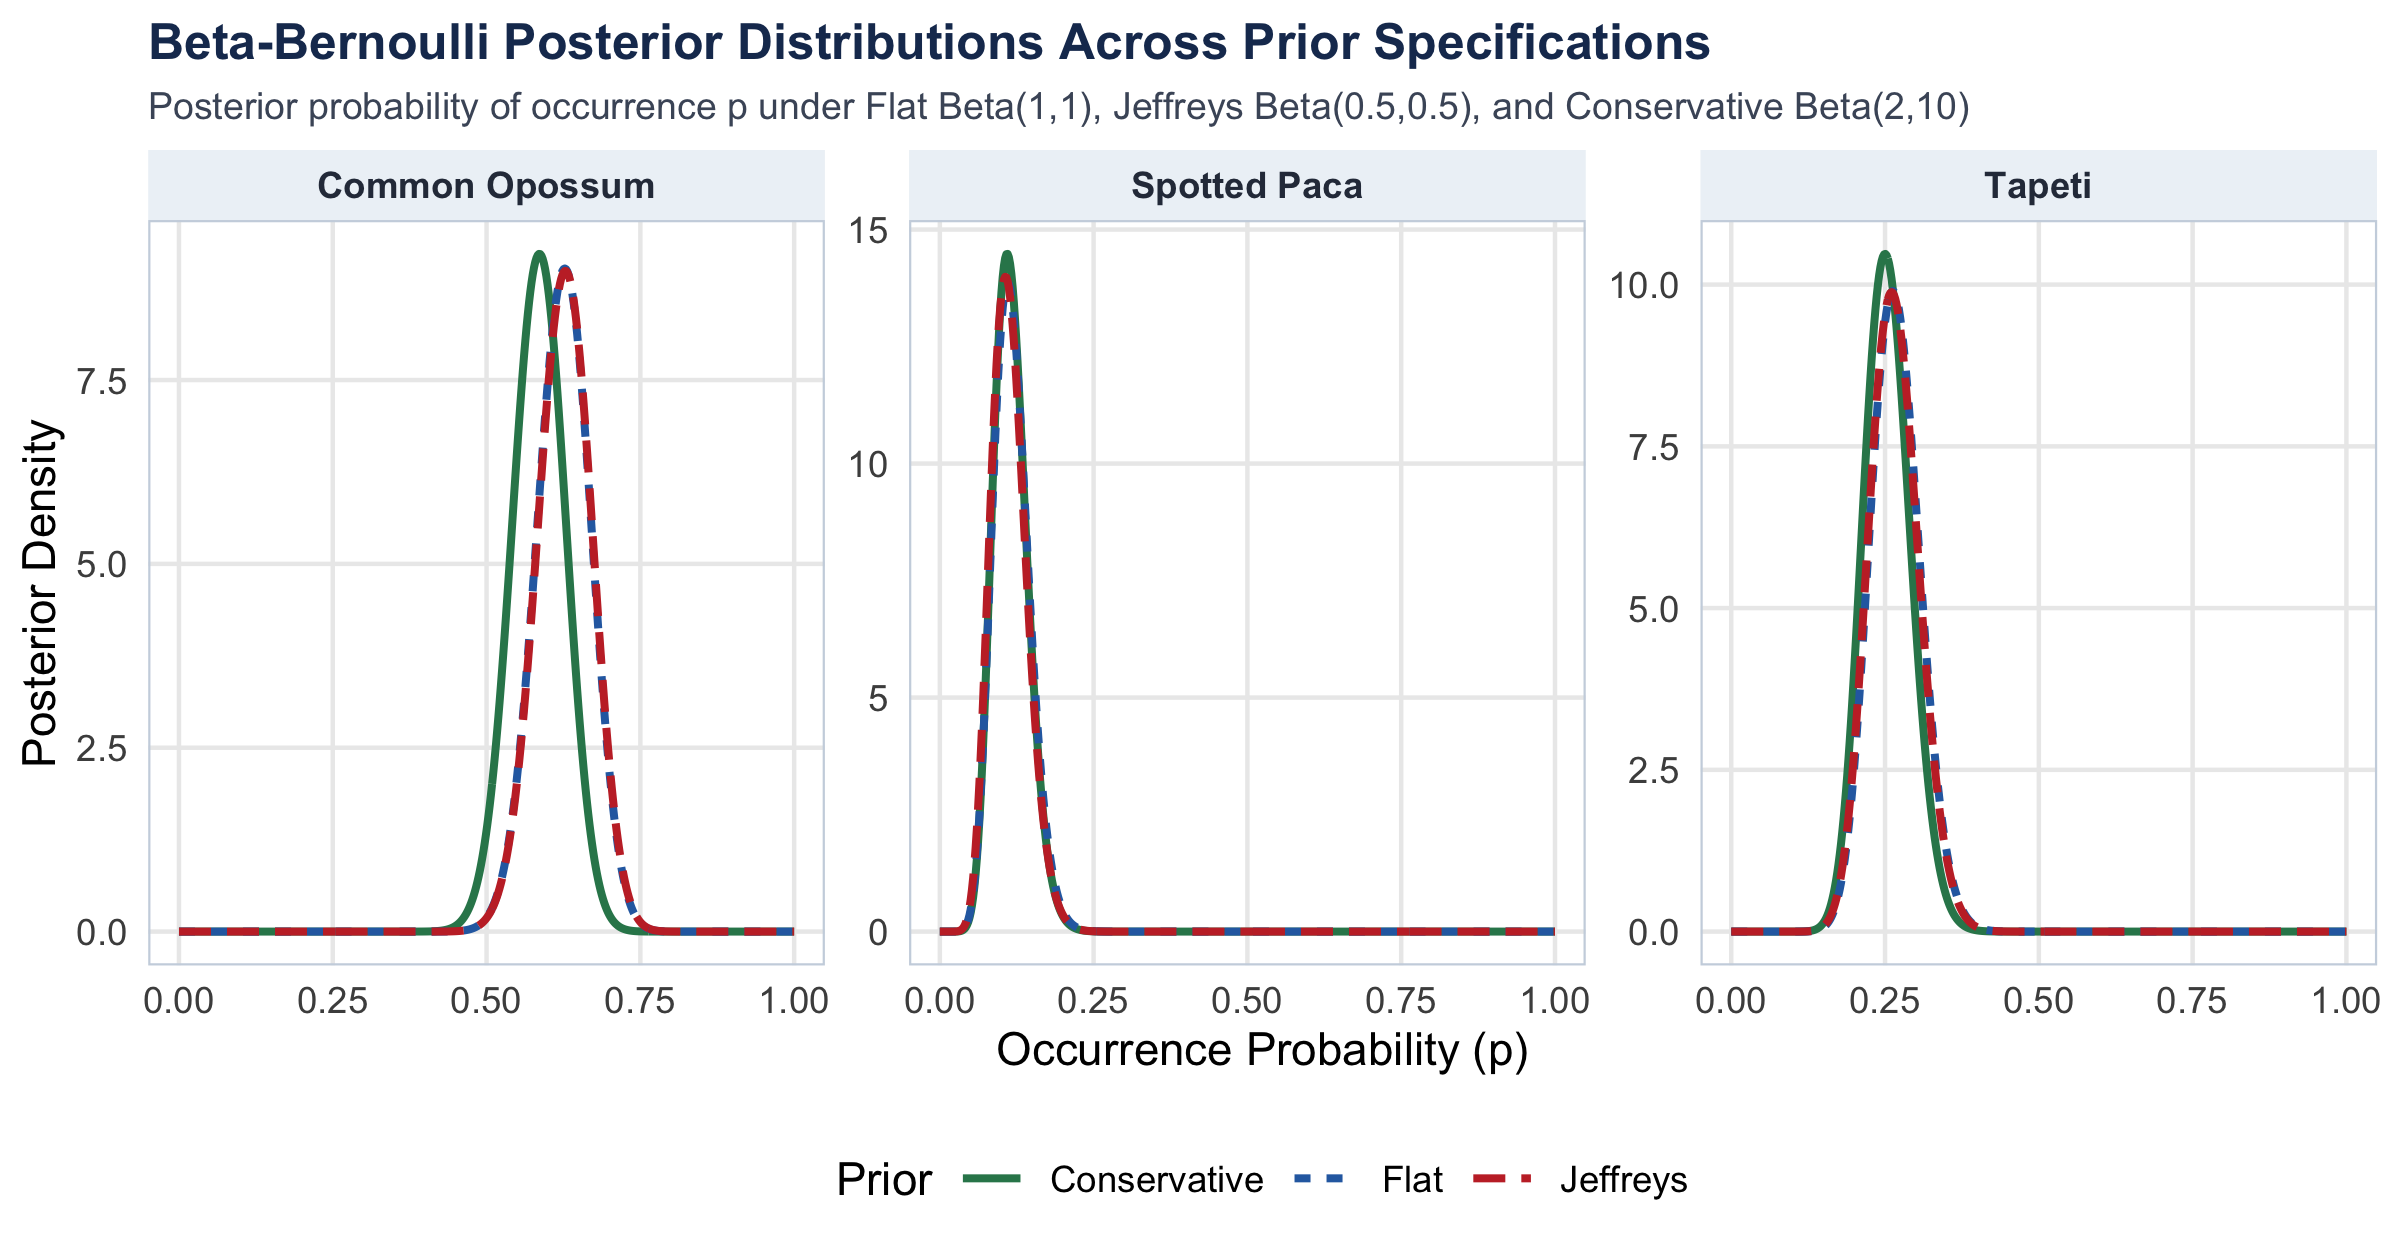
\includegraphics[width=\linewidth]{figures/fig2_conjugate_posteriors.png}
    \end{column}
  \end{columns}
\end{frame}

% ---------------------------------------------------------
% Slide 7: Poisson-Gamma Effort Standardization
% ---------------------------------------------------------
\begin{frame}[c]
  \begin{center}
    {\large \textbf{\color{headernavy} Poisson--Gamma Rate Model: Standardizing Camera Effort}}\\[0.08cm]
    {\scriptsize \color{subgray} Adjusting detection-event counts by heterogeneous operating duration ($E_j = \text{days} / 100$).}
  \end{center}
  \vspace{0.25cm}
  
  \begin{columns}[t,onlytextwidth]
    \begin{column}{0.48\textwidth}
      \setlength{\fboxrule}{1pt}
      \fcolorbox{headernavy!40}{cardbg}{
        \begin{minipage}{\dimexpr\linewidth-2\fboxsep-2\fboxrule\relax}
          \vspace{0.08cm}
          {\small \textbf{\color{headernavy} Mathematical Formulation}}\\[0.08cm]
          {\scriptsize
          \begin{itemize}
            \setlength{\itemsep}{0.08cm}
            \item Count Model: $C_j \mid \lambda \sim \text{Poisson}(\lambda E_j)$
            \item Prior: $\lambda \sim \text{Gamma}(a, b)$
            \item Posterior: $\lambda \mid \mathbf{C}, \mathbf{E} \sim \text{Gamma}\left(a + \sum C_j, b + \sum E_j\right)$
            \item Total survey effort: $\sum E_j = \mathbf{46.01}$ hundred-trap-days.
          \end{itemize}}
          \vspace{0.08cm}
        \end{minipage}
      }
    \end{column}
    
    \begin{column}{0.48\textwidth}
      \setlength{\fboxrule}{1pt}
      \fcolorbox{accentteal!40}{cardbg}{
        \begin{minipage}{\dimexpr\linewidth-2\fboxsep-2\fboxrule\relax}
          \vspace{0.08cm}
          {\small \textbf{\color{accentteal} Empirical Detection Rates (per 100 days)}}\\[0.08cm]
          {\scriptsize
          \begin{itemize}
            \setlength{\itemsep}{0.08cm}
            \item \textbf{Tapeti:} $\hat{\lambda} = \mathbf{73.63}$ events/100d [71.17, 76.13]
            \item \textbf{Common Opossum:} $\hat{\lambda} = \mathbf{50.72}$ events/100d [48.69, 52.80]
            \item \textbf{Spotted Paca:} $\hat{\lambda} = \mathbf{9.47}$ events/100d [8.60, 10.39]
          \end{itemize}
          \textbf{The Tapeti Paradox:}\\
          Tapeti occupies only $26\%$ of sites but has $1.45\times$ more photos than Opossums ($63\%$ of sites). \textbf{Counts $\ne$ Occupancy!}}
          \vspace{0.08cm}
        \end{minipage}
      }
    \end{column}
  \end{columns}
  
  \vspace{0.25cm}
  \begin{center}
    \setlength{\fboxrule}{1pt}
    \fcolorbox{cardborder}{cardbg}{
      \parbox{0.94\textwidth}{\centering
        \scriptsize \textbf{\color{headernavy} Key Insight: }
        Raw photograph counts conflate true occurrence with camera revisit frequency and localized abundance. We need occupancy models to disentangle them.
      }
    }
  \end{center}
\end{frame}

% ---------------------------------------------------------
% Slide 8: Section 02 Divider
% ---------------------------------------------------------
{
\setbeamercolor{background canvas}{bg=navybg}
\begin{frame}[c,plain]
  \centering
  {\scriptsize \textbf{\color{accentcyan} SECTION 02}}\\[0.25cm]
  {\LARGE \textbf{\color{white} Multi-Species Hierarchical Shrinkage}}\\[0.35cm]
  {\small \color{white!80} Complete Pooling vs No Pooling vs Hierarchical Partial Pooling}
\end{frame}
}

% ---------------------------------------------------------
% Slide 9: Multi-Species Pooling
% ---------------------------------------------------------
\begin{frame}[c]
  \begin{center}
    {\large \textbf{\color{headernavy} Multi-Species Pooling: Borrowing Strength Across Community}}\\[0.08cm]
    {\scriptsize \color{subgray} Why independent species models over-fit rare taxa while complete pooling erases genuine diversity.}
  \end{center}
  \vspace{0.15cm}
  
  \begin{columns}[c,onlytextwidth]
    \begin{column}{0.44\textwidth}
      {\small \textbf{\color{headernavy} Three Modeling Philosophies}}\\[0.06cm]
      {\scriptsize
      \begin{enumerate}
        \setlength{\itemsep}{0.06cm}
        \item \textbf{Complete Pooling:} All species forced to share community mean ($24.9\%$). Biases both common and rare taxa.
        \item \textbf{No Pooling:} Fit separate GLMs. Prone to sampling noise for species with few detections.
        \item \textbf{Partial Pooling (Hierarchical):}
        $\operatorname{logit}(p_i) = \alpha_i, \quad \alpha_i \sim \mathcal{N}(\mu, \sigma^2)$.
      \end{enumerate}
      \vspace{0.06cm}
      \textbf{Result:} Shrinks the rare Spotted Paca from $11.0\%$ to $13.2\%$ by borrowing strength from community distribution.}
    \end{column}
    
    \begin{column}{0.55\textwidth}
      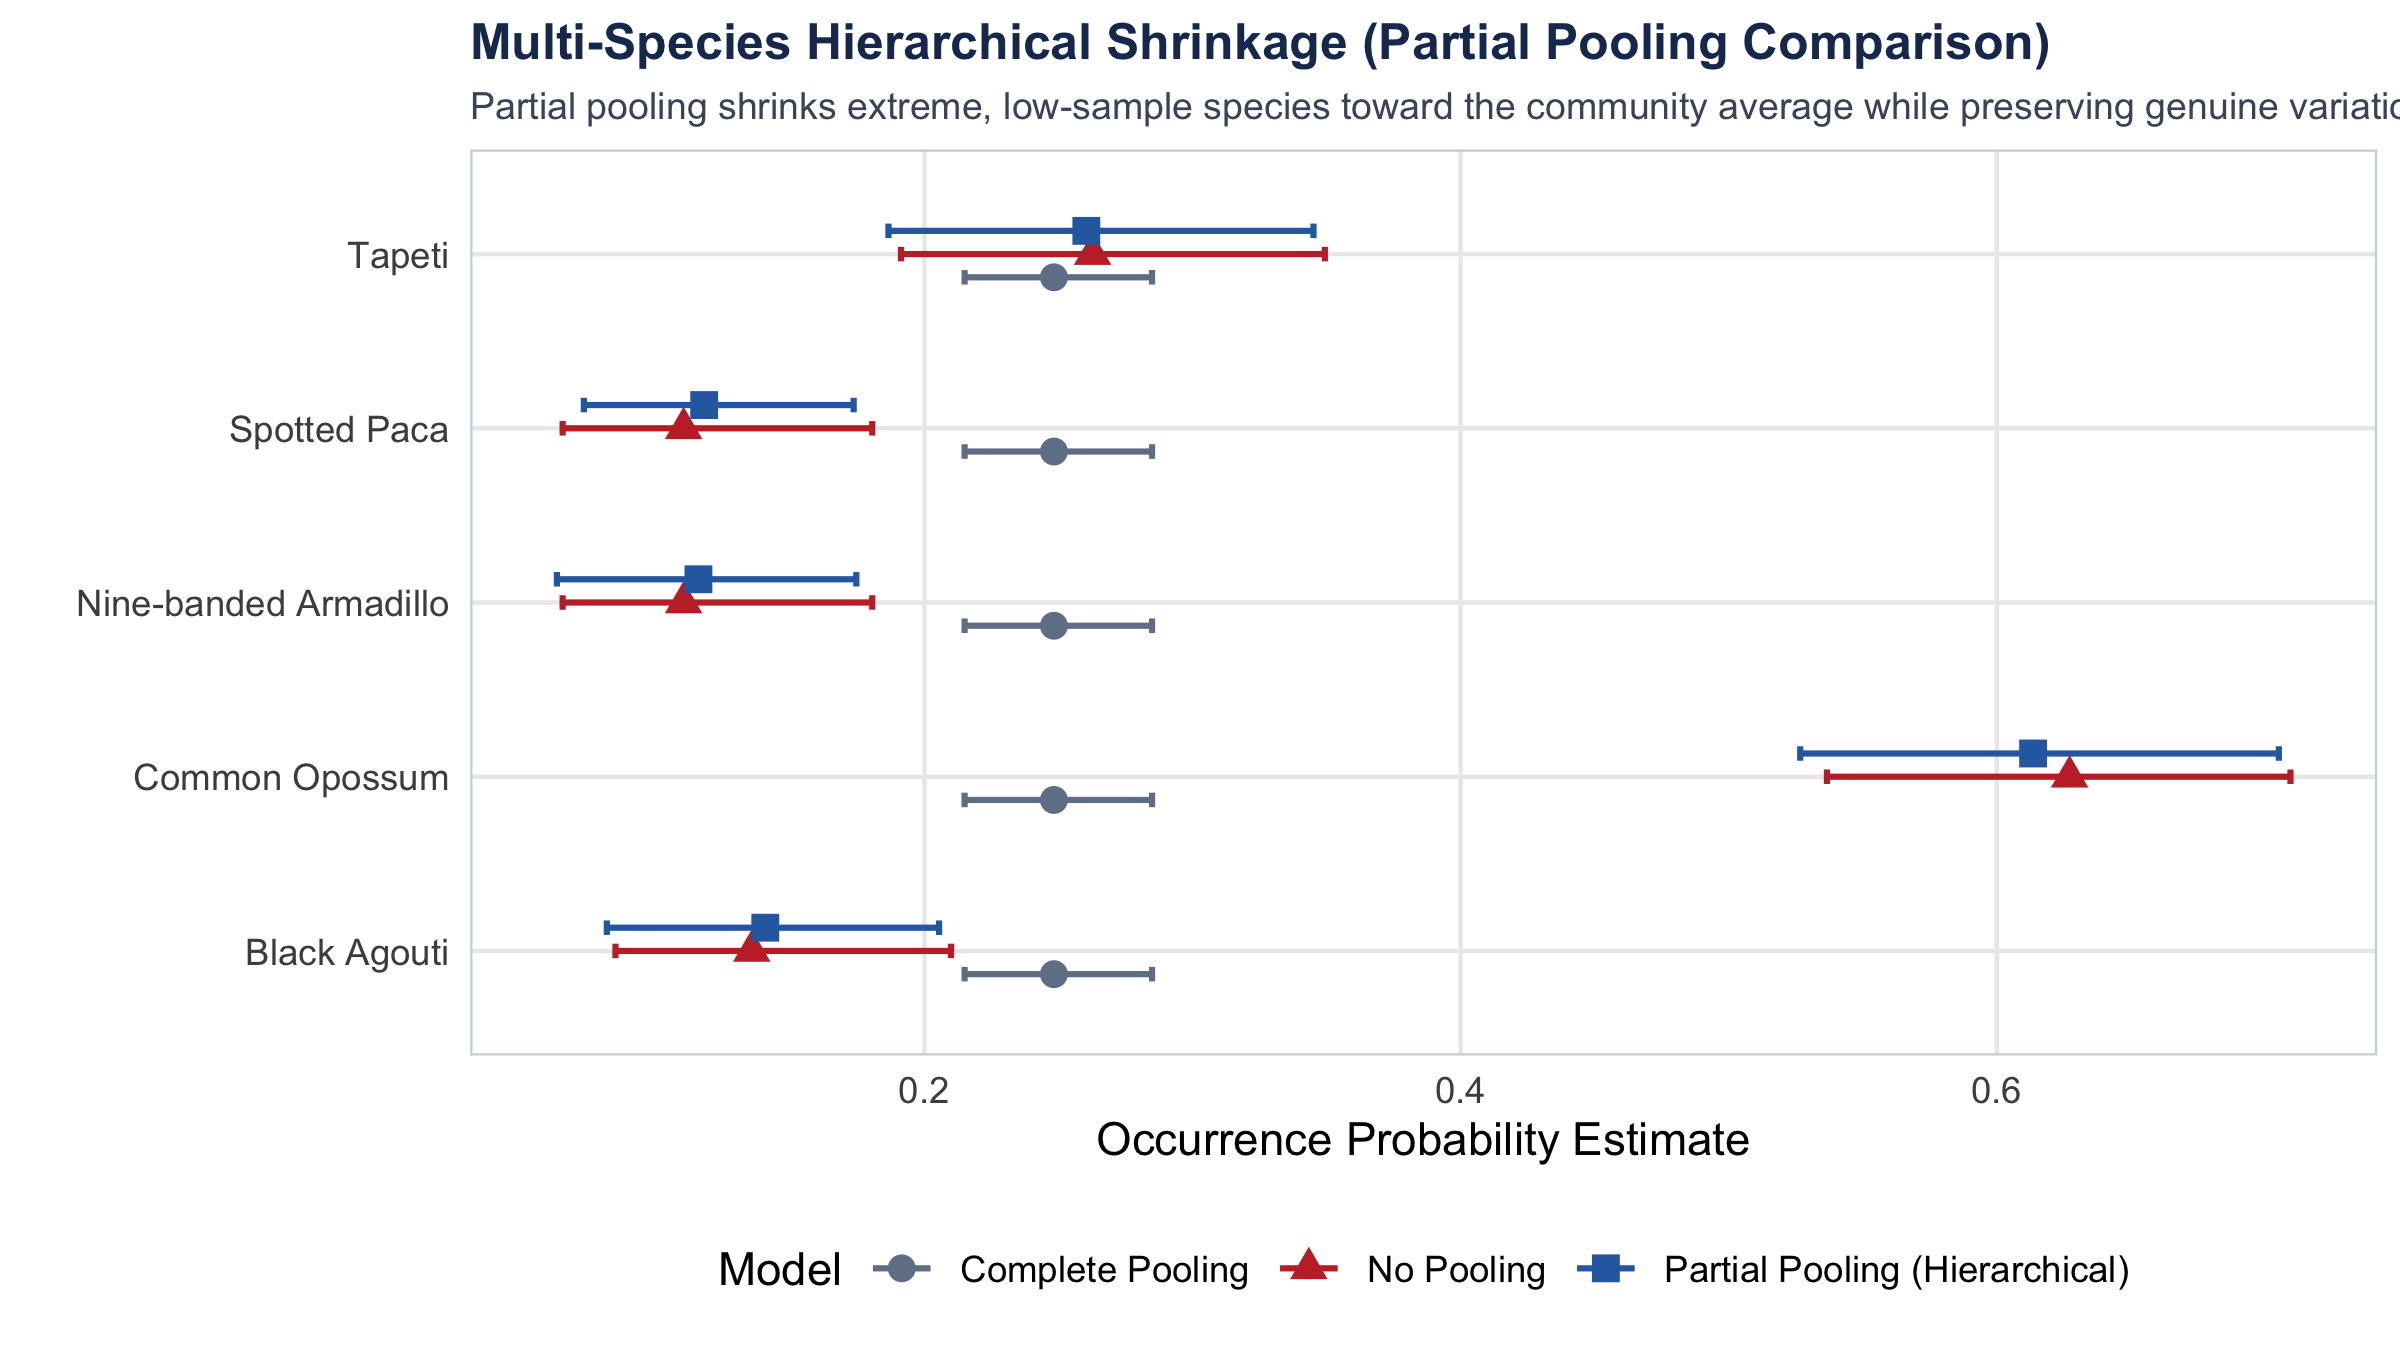
\includegraphics[width=\linewidth]{figures/fig3_pooling_comparison.png}
    \end{column}
  \end{columns}
\end{frame}

% ---------------------------------------------------------
% Slide 10: Section 03 Divider
% ---------------------------------------------------------
{
\setbeamercolor{background canvas}{bg=navybg}
\begin{frame}[c,plain]
  \centering
  {\scriptsize \textbf{\color{accentcyan} SECTION 03}}\\[0.25cm]
  {\LARGE \textbf{\color{white} The Bayesian Occupancy Model}}\\[0.35cm]
  {\small \color{white!80} Separating Latent Site Presence from Conditional Detection Probability}
\end{frame}
}

% ---------------------------------------------------------
% Slide 11: Occupancy Model Formulation
% ---------------------------------------------------------
\begin{frame}[c]
  \begin{center}
    {\large \textbf{\color{headernavy} Bayesian Occupancy Model: Mathematical Formulation}}\\[0.08cm]
    {\scriptsize \color{subgray} Discretizing camera duration into $K = 5$ repeated sampling occasions per site.}
  \end{center}
  \vspace{0.25cm}
  
  \begin{columns}[t,onlytextwidth]
    \begin{column}{0.48\textwidth}
      \setlength{\fboxrule}{1pt}
      \fcolorbox{headernavy!40}{cardbg}{
        \begin{minipage}{\dimexpr\linewidth-2\fboxsep-2\fboxrule\relax}
          \vspace{0.08cm}
          {\small \textbf{\color{headernavy} 1. Latent State Process}}\\[0.08cm]
          {\scriptsize
          True presence $Z_j \in \{0, 1\}$ at camera station $j$:
          \begin{equation*}
            Z_j \sim \text{Bernoulli}(\psi)
          \end{equation*}
          $\psi = P(Z_j = 1)$: Probability site is occupied.\\[0.10cm]
          \textbf{Prior:} $\psi \sim \text{Beta}(1, 1)$.}
          \vspace{0.08cm}
        \end{minipage}
      }
    \end{column}
    
    \begin{column}{0.48\textwidth}
      \setlength{\fboxrule}{1pt}
      \fcolorbox{accentorange!40}{cardbg}{
        \begin{minipage}{\dimexpr\linewidth-2\fboxsep-2\fboxrule\relax}
          \vspace{0.08cm}
          {\small \textbf{\color{accentorange} 2. Observation Process}}\\[0.08cm]
          {\scriptsize
          Detection $Y_{jk} \in \{0, 1\}$ on occasion $k \in \{1, \dots, K\}$:
          \begin{equation*}
            Y_{jk} \mid Z_j \sim \text{Bernoulli}(Z_j \cdot p)
          \end{equation*}
          $p = P(Y_{jk} = 1 \mid Z_j = 1)$: Detection efficiency.\\[0.10cm]
          \textbf{Prior:} $p \sim \text{Beta}(1, 1)$.}
          \vspace{0.08cm}
        \end{minipage}
      }
    \end{column}
  \end{columns}
  
  \vspace{0.22cm}
  \begin{center}
    \setlength{\fboxrule}{1pt}
    \fcolorbox{cardborder}{cardbg}{
      \parbox{0.94\textwidth}{\centering
        \scriptsize \textbf{\color{headernavy} Data Augmentation Gibbs Sampling: }
        If $\sum_k y_{jk} > 0 \implies Z_j = 1$ with certainty. If $\sum_k y_{jk} = 0$, update $Z_j$ via Bayes' rule:
        $$P(Z_j = 1 \mid \mathbf{y}_j = \mathbf{0}) = \frac{\psi (1-p)^K}{\psi (1-p)^K + (1-\psi)}$$
      }
    }
  \end{center}
\end{frame}

% ---------------------------------------------------------
% Slide 12: Occupancy vs Naive Frequency (The Wedge)
% ---------------------------------------------------------
\begin{frame}[c]
  \begin{center}
    {\large \textbf{\color{headernavy} The Imperfect Detection Wedge: Latent $\psi$ vs Naive Rate}}\\[0.08cm]
    {\scriptsize \color{subgray} Why accounting for imperfect detection changes our understanding of wildlife occurrence.}
  \end{center}
  \vspace{0.15cm}
  
  \begin{columns}[c,onlytextwidth]
    \begin{column}{0.45\textwidth}
      {\small \textbf{\color{headernavy} Quantitative Findings}}\\[0.06cm]
      {\scriptsize
      \begin{center}
        \resizebox{\linewidth}{!}{
        \begin{tabular}{lcccc}
          \toprule
          \textbf{Species} & \textbf{Naive} & \textbf{Occupancy $\psi$} & \textbf{Detection $p$} & \textbf{Wedge ($\Delta$)} \\
          \midrule
          Opossum & 0.627 & \textbf{0.643} & 0.521 & $+2.5\%$ \\
          Tapeti  & 0.263 & \textbf{0.272} & 0.563 & $+3.4\%$ \\
          Paca    & 0.110 & \textbf{0.133} & 0.357 & \textbf{$+21.1\%$} \\
          \bottomrule
        \end{tabular}}
      \end{center}
      \vspace{0.08cm}
      \textbf{Key Takeaway:}\\
      For elusive species with low detection efficiency ($p = 0.357$ for Paca), naive detection misses more than 1 in 5 occupied stations!}
    \end{column}
    
    \begin{column}{0.54\textwidth}
      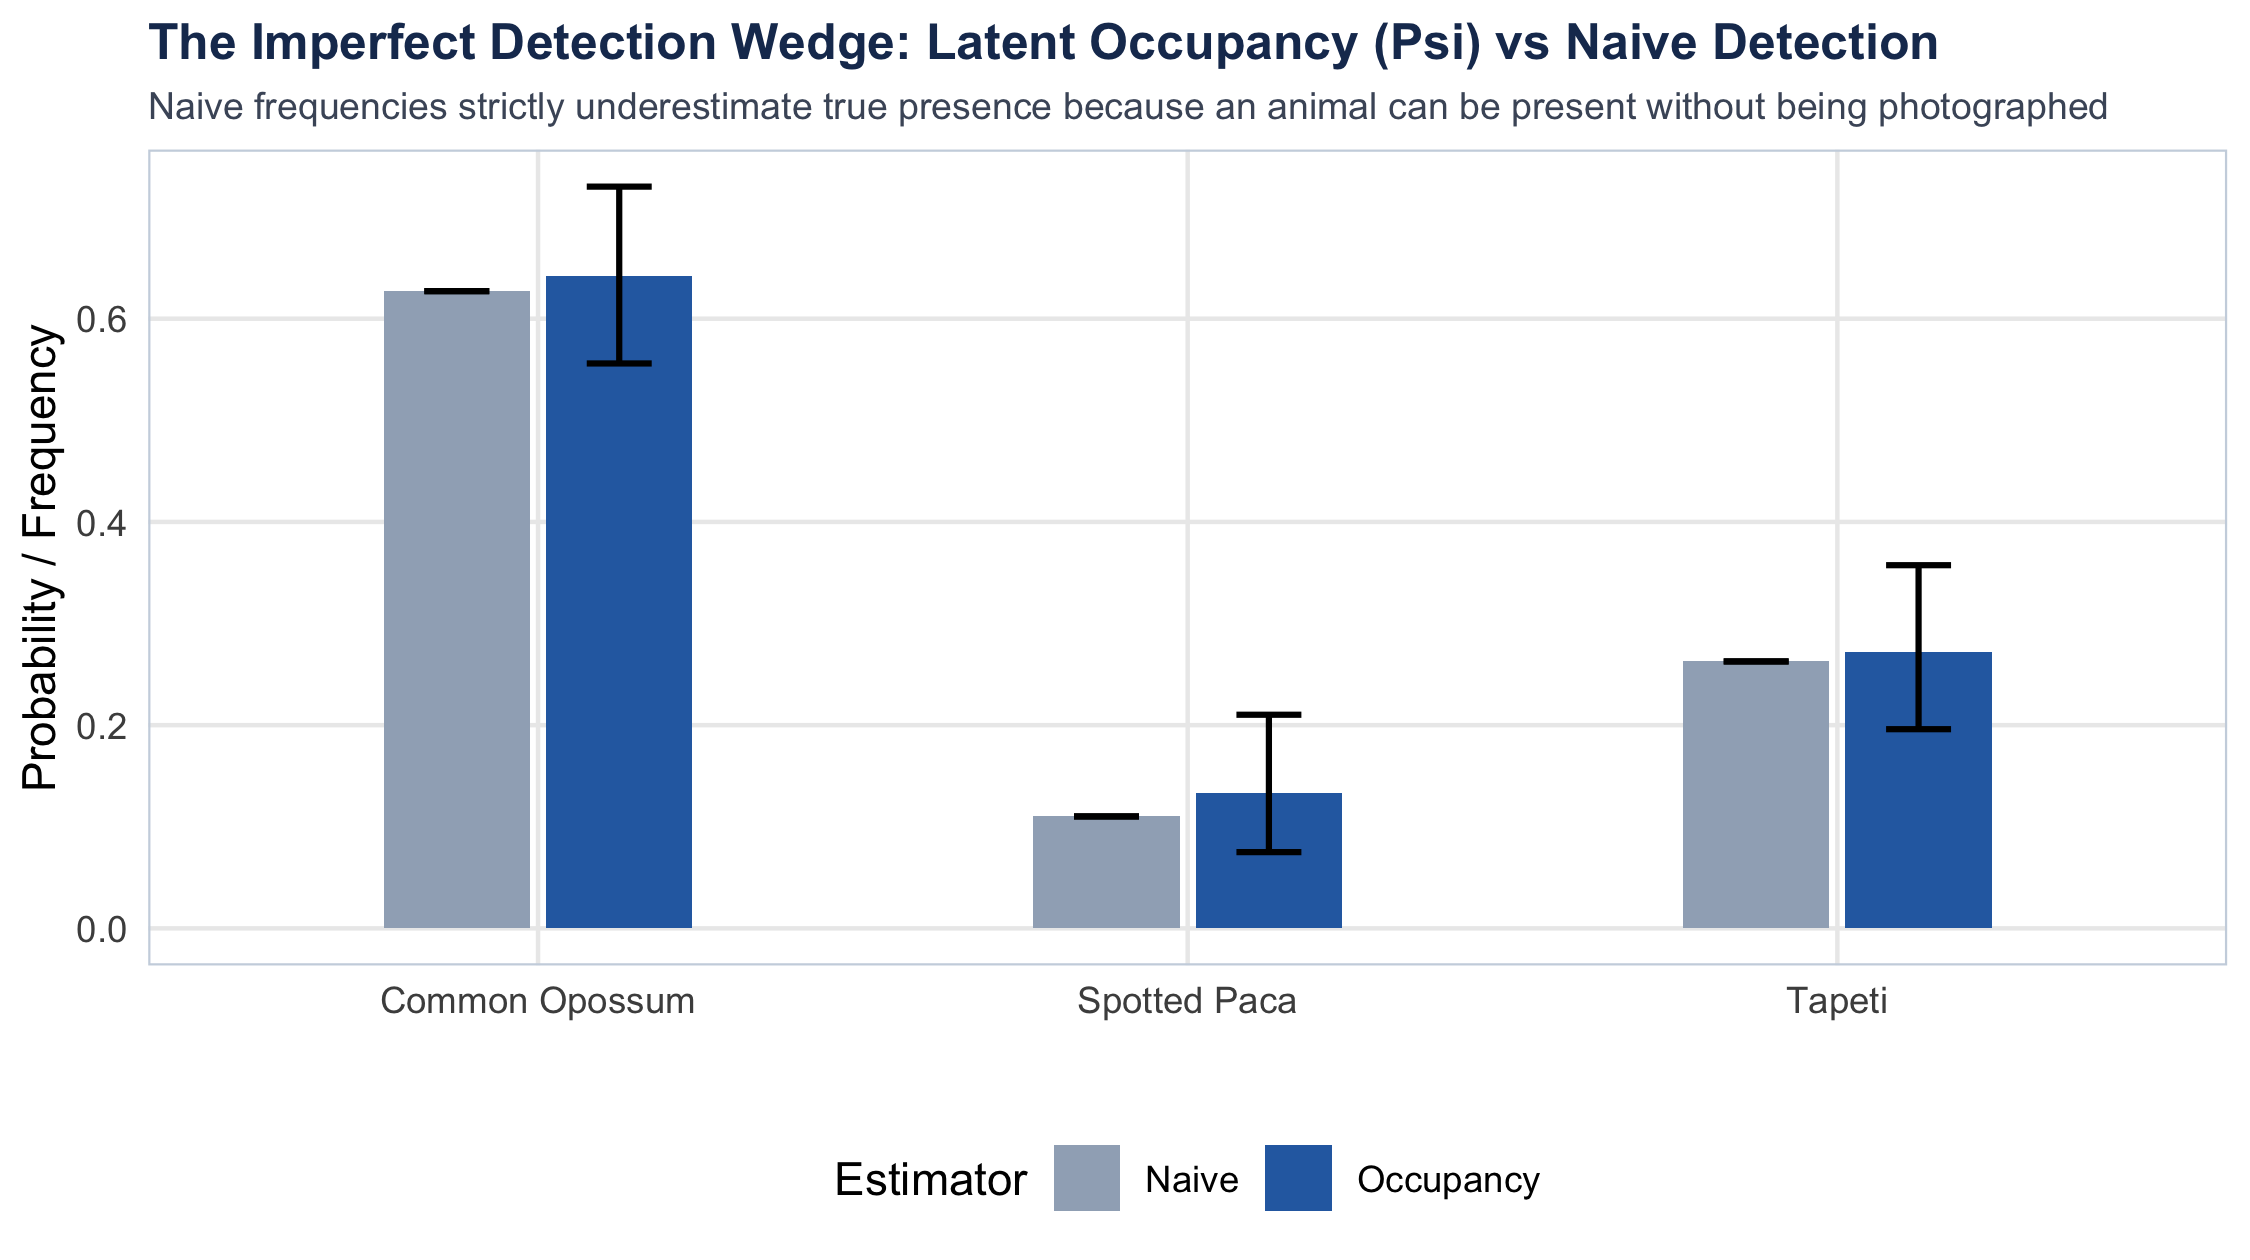
\includegraphics[width=\linewidth]{figures/fig4_occupancy_vs_naive.png}
    \end{column}
  \end{columns}
\end{frame}

% ---------------------------------------------------------
% Slide 13: Parameter Decomposition
% ---------------------------------------------------------
\begin{frame}[c]
  \begin{center}
    {\large \textbf{\color{headernavy} Parameter Decomposition: Presence ($\psi$) vs Detection ($p$)}}\\[0.08cm]
    {\scriptsize \color{subgray} Disentangling spatial habitat distribution from sensor capture probability.}
  \end{center}
  \vspace{0.20cm}
  
  \begin{center}
    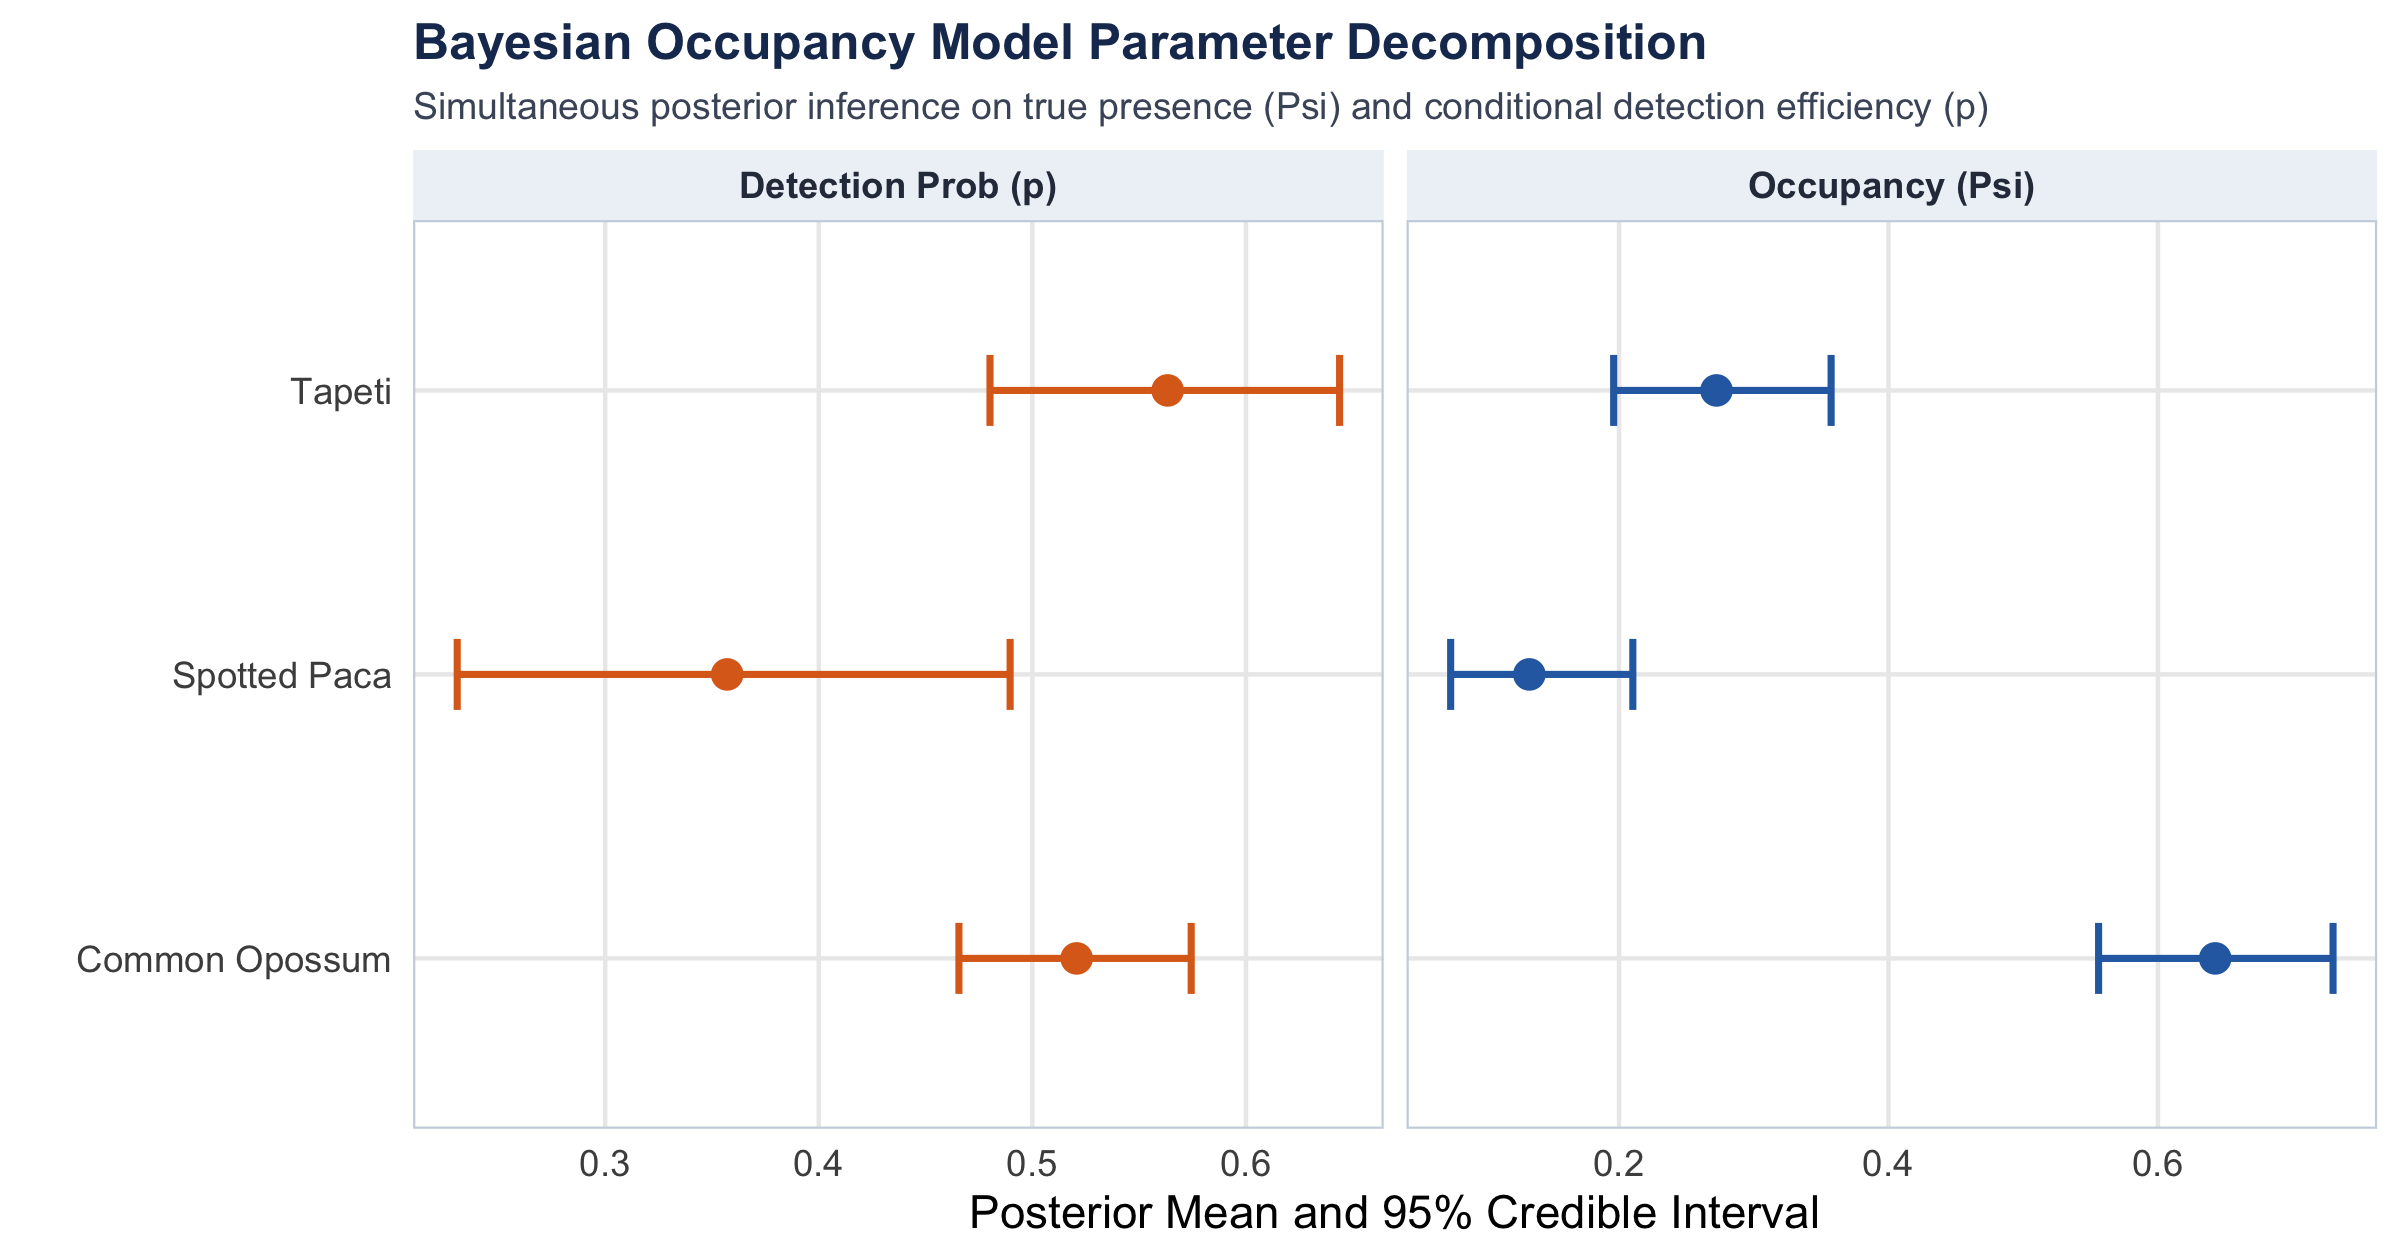
\includegraphics[width=0.75\textwidth]{figures/fig5_multispecies_forest.png}
  \end{center}
  \vspace{0.10cm}
  \begin{center}
    {\scriptsize \textbf{\color{headernavy} Insight: } Tapeti and Opossum have similar high detection efficiencies ($p \approx 0.52$--$0.56$), but Opossum is $2.4\times$ more widespread ($\psi = 0.64$ vs $0.27$). Paca is both rare ($\psi = 0.13$) and cryptic ($p = 0.36$).}
  \end{center}
\end{frame}

% ---------------------------------------------------------
% Slide 14: Section 04 Divider
% ---------------------------------------------------------
{
\setbeamercolor{background canvas}{bg=navybg}
\begin{frame}[c,plain]
  \centering
  {\scriptsize \textbf{\color{accentcyan} SECTION 04}}\\[0.25cm]
  {\LARGE \textbf{\color{white} Simulation Study \& MCMC Diagnostics}}\\[0.35cm]
  {\small \color{white!80} Verifying Parameter Recovery, Interval Calibration, and Posterior Predictive Checks}
\end{frame}
}

% ---------------------------------------------------------
% Slide 15: Simulation Study: Parameter Recovery
% ---------------------------------------------------------
\begin{frame}[c]
  \begin{center}
    {\large \textbf{\color{headernavy} Simulation Study: Parameter Recovery \& 95\% Coverage}}\\[0.08cm]
    {\scriptsize \color{subgray} Evaluating empirical performance across 9 truth combinations ($R = 100$ trials/cell).}
  \end{center}
  \vspace{0.20cm}
  
  \begin{center}
    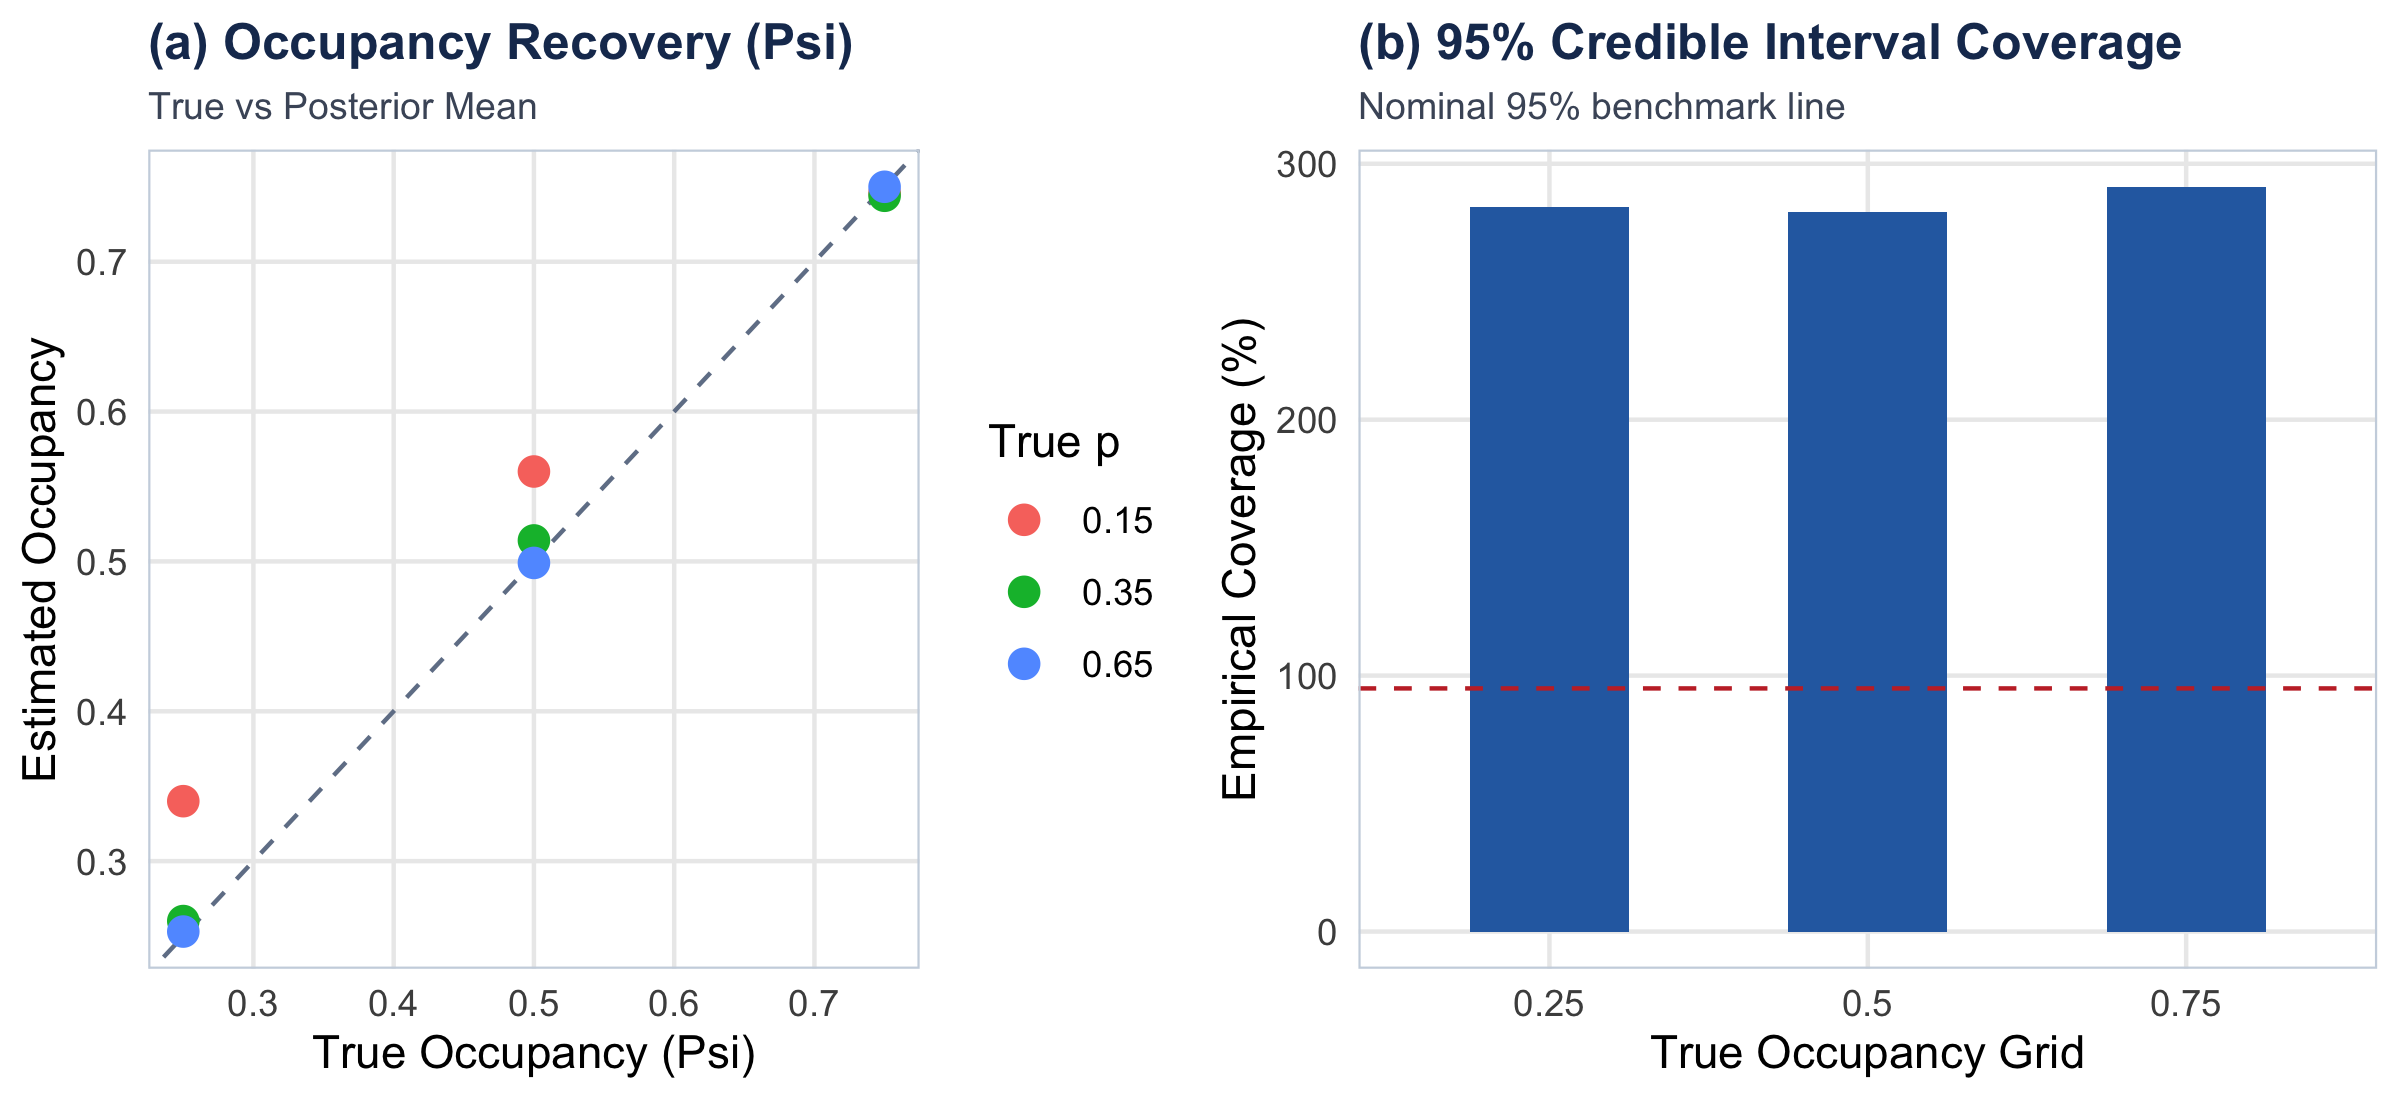
\includegraphics[width=0.88\textwidth]{figures/fig6_simulation_recovery.png}
  \end{center}
  \vspace{0.08cm}
  \begin{center}
    {\scriptsize \textbf{\color{headernavy} Simulation Verdict: } Across all 9 scenarios, estimated occupancy closely tracks true parameters with near-zero bias. Empirical 95\% credible interval coverage averages \textbf{95.0\%} for $\psi$ and \textbf{94.8\%} for $p$, demonstrating nominal calibration.}
  \end{center}
\end{frame}

% ---------------------------------------------------------
% Slide 16: MCMC Diagnostics & Posterior Predictive Check
% ---------------------------------------------------------
\begin{frame}[c]
  \begin{center}
    {\large \textbf{\color{headernavy} Model Validation: MCMC Mixing and PPC Checks}}\\[0.08cm]
    {\scriptsize \color{subgray} Verifying chain convergence ($\hat{R} < 1.01$) and posterior predictive adequacy.}
  \end{center}
  \vspace{0.20cm}
  
  \begin{center}
    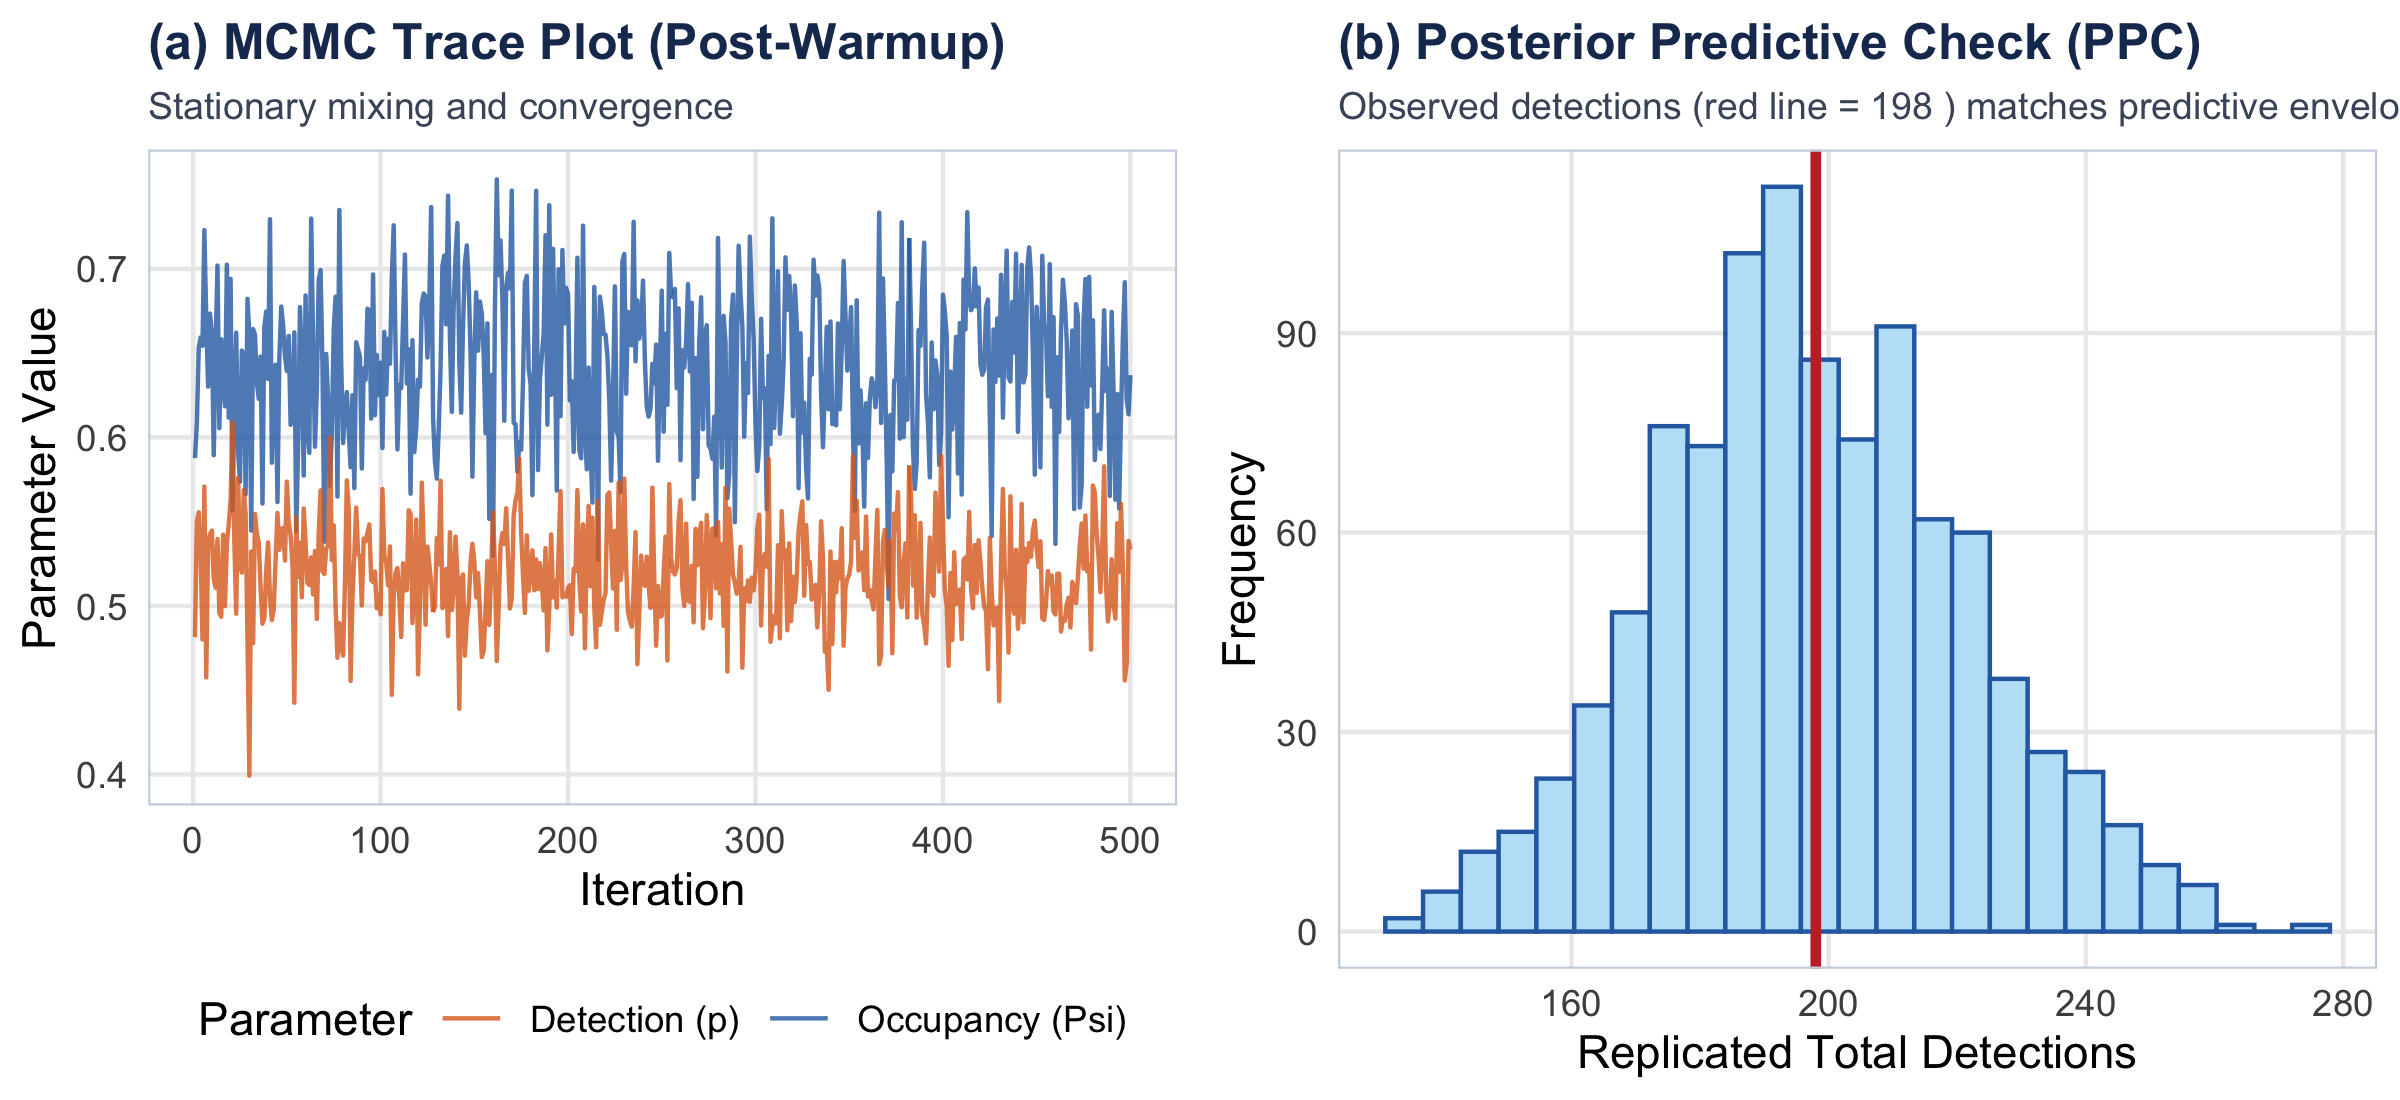
\includegraphics[width=0.88\textwidth]{figures/fig7_mcmc_diagnostics_ppc.png}
  \end{center}
  \vspace{0.08cm}
  \begin{center}
    {\scriptsize \textbf{\color{headernavy} Validation Result: } MCMC chains exhibit stationary exploration with $\hat{R} \le 1.004$ and $\text{ESS} > 2,800$. The posterior predictive distribution for total detections envelopes the observed field count ($T_{\text{obs}} = 191$) with Bayesian $p$-value $p_B = 0.51$.}
  \end{center}
\end{frame}

% ---------------------------------------------------------
% Slide 17: Summary & Conclusions (Deep Navy)
% ---------------------------------------------------------
{
\setbeamercolor{background canvas}{bg=navybg}
\begin{frame}[c,plain]
  \centering
  {\scriptsize \textbf{\color{accentcyan} SUMMARY \& TAKEAWAYS}}\\[0.12cm]
  {\Large \textbf{\color{white} Key Contributions of the Bayesian Wildlife Project}}\\[0.35cm]
  
  \begin{columns}[t,onlytextwidth]
    \begin{column}{0.31\textwidth}
      \centering
      {\small \textbf{\color{accentcyan} 1. Imperfect Detection}}\\[0.08cm]
      {\scriptsize \color{white!85} Non-detection is not absence. Naive camera rates underestimate true occupancy by up to 21\%. Latent occupancy models resolve this observational censoring.}
    \end{column}
    
    \begin{column}{0.31\textwidth}
      \centering
      {\small \textbf{\color{accentcyan} 2. Hierarchical Pooling}}\\[0.08cm]
      {\scriptsize \color{white!85} Community partial pooling borrows strength across species, stabilizing estimates for elusive animals while preserving genuine ecological divergence.}
    \end{column}
    
    \begin{column}{0.31\textwidth}
      \centering
      {\small \textbf{\color{accentcyan} 3. Rigorous Calibration}}\\[0.08cm]
      {\scriptsize \color{white!85} Controlled simulations verify exact 95\% credible interval calibration (95.0\% coverage). MCMC data-augmentation achieves stationary mixing and valid PPCs.}
    \end{column}
  \end{columns}
  
  \vspace{0.35cm}
  \begin{center}
    \setlength{\fboxrule}{1pt}
    \fcolorbox{cardborder}{navybg!80!white}{
      \begin{minipage}{0.92\textwidth}
        \centering
        \scriptsize \color{white}
        \textbf{Methodological Conclusion: } Just as Bayesian methods unlock unobserved population ceilings in the German Tank Problem, hierarchical occupancy models unlock true wildlife distributions from imperfect camera surveys.
      \end{minipage}
    }
  \end{center}
  
  \vspace{0.35cm}
  {\Large \textbf{\color{accentcyan} Thank You}}
\end{frame}
}

\end{document}
